\documentclass[12pt, twoside]{article}
\documentclass[12pt, twoside]{article}
\usepackage[letterpaper, margin=1in, headsep=0.2in]{geometry}
\setlength{\headheight}{0.6in}
%\usepackage[english]{babel}
\usepackage[utf8]{inputenc}
\usepackage{microtype}
\usepackage{amsmath}
\usepackage{amssymb}
%\usepackage{amsfonts}
\usepackage{siunitx} %units in math. eg 20\milli\meter
\usepackage{yhmath} % for arcs, overparenth command
\usepackage{tikz} %graphics
\usetikzlibrary{quotes, angles}
\usepackage{graphicx} %consider setting \graphicspath{{images/}}
\usepackage{parskip} %no paragraph indent
\usepackage{enumitem}
\usepackage{multicol}
\usepackage{venndiagram}

\usepackage{fancyhdr}
\pagestyle{fancy}
\fancyhf{}
\renewcommand{\headrulewidth}{0pt} % disable the underline of the header
\raggedbottom
\hfuzz=2mm %suppresses overfull box warnings

\usepackage{hyperref}
\usepackage{float}

\title{Algebra 2}
\author{Chris Huson}
\date{December 2023}

%\fancyhead[LE]{\thepage}
\fancyhead[RO]{\thepage \\ Name: \hspace{4cm} \,\\}
\fancyhead[LO]{BECA / Huson / Algebra 2: Polynomials \\* 1 December 2023}

\begin{document}

\subsubsection*{2.15 Quiz: Quadratic functions and review}
\begin{enumerate}

\newpage
\setcounter{enumi}{8} % Restart numbering at 9
\subsubsection*{A2-F.IF.7c Graph polynomials, identify zeros, end behavior}
\item The polynomial $f(x)$ is graphed below. 
\begin{multicols}{2}
    \begin{enumerate}[itemsep=0.6cm]
        \item What is the degree of the function?
        \item What are zeros of the function?
        \item What factor has a multiplicity of 2?
        \item Write down the $y$-intercept as an ordered pair.
        \item Is the leading coefficient positive, negative, or zero?
        \item Describe the end behavior.
    \end{enumerate} \vspace{1cm} \;

    \columnbreak

    \begin{tikzpicture}[xscale=0.7, yscale=0.8]
        \draw[lightgray,very thin] (-4,-4) grid (4,5);
        \draw [thick, ->] (-4.2,0) -- (4.4,0) node [above] {$x$};
        \draw [thick, ->] (0,-4.2)--(0,5.5) node [right] {$y$};
        \foreach \x in {-4,4} \draw (\x cm,5pt) -- (\x cm,-5pt) node[below] {$\x$};
        \draw (5pt,5 cm) -- (-5pt,5 cm) node[left] {$50$};
        \draw [thick, <->,smooth,samples=20,domain=-3:3.3] plot(\x,{0.25*(\x-1)*(\x-3)*(\x+2)^2});
    \end{tikzpicture}
\end{multicols}

\subsubsection*{A2-F.BF.2 Write arithmetic and geometric sequences with recursive formulas}
\item Write a recursive definition of the sequence $a_1 = 3$, $a_2 = 8$, $a_3 = 13$, $a_4 = 18, \ldots$  \vspace{3cm}

\item Find the difference $f(x)-g(x)$ as a polynomial in standard form, given \\[0.25cm]
    $f(x)=4x^4+5x^3-3x$ and $g(x)=2x^3-2x^2-3x-1$.

\end{enumerate}
\end{document}